\paragraph{QuizziPedia::Back-End::App::Models::QuizModel}
\label{QuizziPedia::Back-End::App::Models::QuizModel}
\begin{figure}[ht]
	\centering
	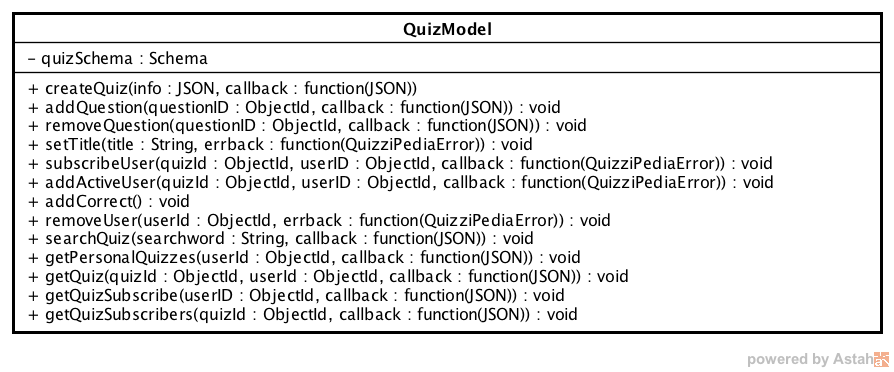
\includegraphics[scale=0.45]{UML/Classi/Back-End/QuizziPedia_Back-End_App_Models_quizModel.png}
	\caption{QuizziPedia::Back-End::App::Models::QuizModel}
\end{figure}
\FloatBarrier



\begin{itemize}
	\item \textbf{Descrizione} \\
	Classe che modella i questionari all'interno dell'applicazione.
	\item \textbf{Utilizzo} \\
	Viene utilizzata per rappresentare i dati relativi ai questionari all'interno dell'applicazione. Si interfaccia con la libreria \textit{Mongoose\ped{G}} per la creazione dello schema e dei relativi metodi statici o di istanza.
	\item \textbf{Relazioni con altre classi}
		\begin{itemize}
			\item \textbf{OUT} \texttt{QuestionModel}\\
			Classe che rappresenta le operazioni relative alle domande.
			\item \textbf{OUT} \texttt{UserModel}\\
			Classe che rappresenta le operazioni relative agli utenti.
		\end{itemize}
	\item \textbf{Attributi}
		\begin{itemize}
			\item \textbf{- quizSchema: Schema} \\
			Questo campo dati rappresenta lo schema \textit{Mongoose\ped{G}} dei quiz di \progetto. Lo schema prevede i seguenti attributi:
				\begin{itemize}
					\item \texttt{title} di tipo \texttt{String}, rappresenta il titolo del questionario;
					\item \texttt{author} di tipo \texttt{ObjectId}, rappresenta il riferimento all'identificativo nel database dell'utente che ha creato il questionario;
					\item \texttt{questions} di tipo \texttt{Array}, contiene oggetti di tipo \texttt{ObjectId} che rappresentano i riferimenti agli identificativi nel database delle domande appartenenti al questionario;
					\item \texttt{registeredUsers} di tipo \texttt{Array}, contiene oggetti di tipo \texttt{ObjectId} che rappresentano i riferimenti agli identificativi nel database degli utenti iscritti al quiz;
					\item \texttt{activeUsers} di tipo \texttt{Array}, contiene oggetti di tipo \texttt{ObjectId} che rappresentano i riferimenti agli identificativi nel database degli utenti che partecipano effettivamente al questionario;
					\item \texttt{correctAnswers} di tipo \texttt{Number}, rappresenta il numero totale di risposte corrette date dagli utenti alle domande del questionario.	
				\end{itemize}
		\end{itemize}
	\item \textbf{Metodi}
		\begin{itemize}
		
			\item \texttt{+ createQuiz(info: JSON, callback: function(JSON), errback: function(QuizziPediaError)): void}\\
			Crea un questionario con i dati che vengono passati.\\
			\textbf{Parametri}:
			\begin{itemize}
				\item \texttt{info: JSON}\\
				Rappresenta i dati del questionario che verrà creato.
				\item \texttt{callback: function(JSON)}\\
				Rappresenta la \textit{callback\ped{G}} che verrà eseguita al termine dell'elaborazione.
				\item \texttt{errback: function(QuizziPediaError)}\\
				Rappresenta la \textit{callback\ped{G}} che verrà eseguita al termine dell'elaborazione in caso di errore.
			\end{itemize}
			
			\item \texttt{+ addQuestion(questionID: ObjectId): void}\\
			Aggiunge una domanda al questionario.\\
			\textbf{Parametri}:
			\begin{itemize}
				\item \texttt{questionID: ObjectId}\\
				Rappresenta l'identificativo della domanda da aggiungere al questionario.
			\end{itemize}
			
			\item \texttt{+ removeQuestion(questionID: ObjectId): void}\\
			Rimuove una domanda dal questionario.\\
			\textbf{Parametri}:
			\begin{itemize}
				\item \texttt{questionID: ObjectId}\\
				Rappresenta l'identificativo della domanda da rimuovere dal questionario.
			\end{itemize}
			
			\item \texttt{+ setTitle(title: String, errback: function(QuizziPediaError)): void}\\ 		
			Dà un titolo al questionario.\\
			\textbf{Parametri}:
			\begin{itemize}
				\item \texttt{title: String}\\
				Rappresenta il titolo da dare al questionario.
				\item \texttt{errback: function(QuizziPediaError)}\\
				Rappresenta la \textit{callback\ped{G}} che verrà eseguita al termine dell'elaborazione in caso di errore.
			\end{itemize}
			
			\item \texttt{+ addUser(userID: ObjectId): void}\\
			Iscrive un utente al questionario.\\
			\textbf{Parametri}:
			\begin{itemize}
				\item \texttt{userID: ObjectId}\\
				Rappresenta l'identificativo dell'utente da aggiungere al questionario.
			\end{itemize}
			
			\item \texttt{+ addActiveUser(userID: ObjectId): void}\\
			Iscrive un utente al questionario.\\
			\textbf{Parametri}:
			\begin{itemize}
				\item \texttt{userID: ObjectId}\\
				Rappresenta l'identificativo dell'utente da aggiungere al questionario.
			\end{itemize}
			
			\item \texttt{+ addCorrect(): void}\\
			Incrementa il numero di risposte corrette date alle domande del questionario.\\			
			
			\item \texttt{+ removeUser(userID: ObjectId, errback: function(QuizziPediaError)): void}\\
			Rimuovere un utente dalla lista degli iscritti al questionario.\\
			\textbf{Parametri}:
			\begin{itemize}
				\item \texttt{userID: ObjectId}\\
				Rappresenta l'identificativo dell'utente da rimuovere dalla lista degli iscritti al questionario.
				\item \texttt{errback: function(QuizziPediaError)}\\
				Rappresenta la \textit{callback\ped{G}} che verrà eseguita al termine dell'elaborazione in caso di errore.
			\end{itemize}
			
			\item \texttt{+ searchQuiz(searchword: String, callback: function(JSON), errback: function(QuizziPediaError)): void}\\
			Ricerca un questionario.\\
			\textbf{Parametri}:
			\begin{itemize}
				\item \texttt{title: String}\\
				Rappresenta il titolo del questionario da ricercare.
				\item \texttt{callback: function(JSON)}\\
				Rappresenta la \textit{callback\ped{G}} che verrà eseguita al termine dell'elaborazione.
				\item \texttt{errback: function(QuizziPediaError)}\\
				Rappresenta la \textit{callback\ped{G}} che verrà eseguita al termine dell'elaborazione in caso di errore.
			\end{itemize}
			
			\item \texttt{+ getQuizzes(userID: ObjectId, callback: function(JSON), errback: function(QuizziPediaError)): void}\\
			Ritorna la cronologia dei questionari svolti da un utente.\\
			\textbf{Parametri}:
			\begin{itemize}
				\item \texttt{userID: ObjectId}\\
				Rappresenta l'identificativo dell'utente per cui si deve mostrare la cronologia dei questionari svolti.
				\item \texttt{callback: function(JSON)}\\
				Rappresenta la \textit{callback\ped{G}} che verrà eseguita al termine dell'elaborazione.
				\item \texttt{errback: function(QuizziPediaError)}\\
				Rappresenta la \textit{callback\ped{G}} che verrà eseguita al termine dell'elaborazione in caso di errore.
			\end{itemize}
		\end{itemize}
\end{itemize}